\section{ \textbf{ساختارها}}

\subsection{\lr{sph-skein-big-context}}
\label{subsec:sph-skein-big-context}
این ساختار مورد نظر برای ذخیره و استفاده از هش است (‌ شامل مقادیری از هش قبلی و مقادیر جدید محاسبه شده ). \\ این ساختار شامل یک آرایه‌ی ۶۴ بیتی از کاراکترهاست که به منظور تراز کردن انواع هش استفاده می‌گردد و  هشت عدد ۶۴ بیتی  که برای ذخیره‌ی ۵۱۲ بیت هش  استفاده می‌شوند  و هم‌چنین شامل دو عدد با نام‌های \lr{ptr, bcount} است که این دو عدد به طور معمول برابر ۰ هستند که همانند \lr{nonce} در پیاده‌سازی وریلاگ آن است.



\subsection{\lr{IV512}}
\label{subsec:IV512}
این ساختار شامل مقادیر اولیه‌ی هش است. یک عدد ۵۱۲ بیتی را برای خوانا بودن در مبنای ۱۶ و در ۸ بلاک ۱۶ بیتی نگاه می‌دارد. این مقدار در برنامه‌ به زبان وریلاگ همان \lr{midstate} است.
\subsection{\lr{UBI-BIG}}
\label{subsec:UBI-BIG}

در این تابع روی دیتای ذخیره شده در بافر عملیات درهم‌سازی انجام شده‌است. این درهم‌سازی برمبنای مقادیر قبلی موجود در $  h_0 $ تا  $ h_7 $ ( که در سری قبلی صدا شدن این تابع مشخص شده‌اند)، دیتا و ورودی‌های \lr{extra} و  \lr{etype} انجام شده‌است. 
در ابتدا سه\lr{ sph-u64 }با اسامی $ t_0 , t_1 , t_2 $ تعریف شده‌اند. \lr{ sph-u64 }جنسی تعریف شده برای متغیرهای ۶۴ بیتی بدون علامت است. سپس متغیری به اسم $ u $ تعریف شده‌ که در ادامه‌ی تابع به عنوان شمارنده در حلقه‌ها استفاده شده‌است. با شروع از \lr{buf} هر هشت عنصر که هر کدام یک بایت هستند توسط \lr{sph-dec64le-aligned} به ۶۴ بیت پشت سر هم تبدیل شده و سپس به$ m_0 $تا $ m_7 $ داده شده‌است.  \lr{sph-dec64le-aligned} یک بیت به عنوان شروع هشت بایت ورودی گرفته سپس هشت بایت را به یک دیکودر داده و ۶۴ بیت خروجی می‌دهد. مقدارهای $ m_0 $ تا $ m_7 $ در $ p_0 $ تا $ p_7 $ ریخته شده‌اند. $ m_0 $ تا $ m_7 $ تا اخر تابع بدون تغییر باقی مانده و مقدارهای اولیه‌ی بخش‌های دیتا هستند.  
سپس مقدار ‌\lr{extra} پس از \lr{cast} به\lr{sph-u64} با مقدار \lr{bcount} با ۶ بیت شیفت به چپ جمع شده و به $ t_0 $ داده شده‌است. سپس مقدار ‌\lr{bcount} ، ۵۸ بیت به راست شیفت داده شده و ‌\lr{etype} هم ۵۵ بیت به چپ شیف داده شده‌است. این مقادیر با هم جمع شده‌‌اند و جمعشان به ‌$ t_1 $ داده شده‌است. مقدار شیفت داده شدن‌ها از روی شکل زیر قابل توجیه‌اند:
\begin{center}
	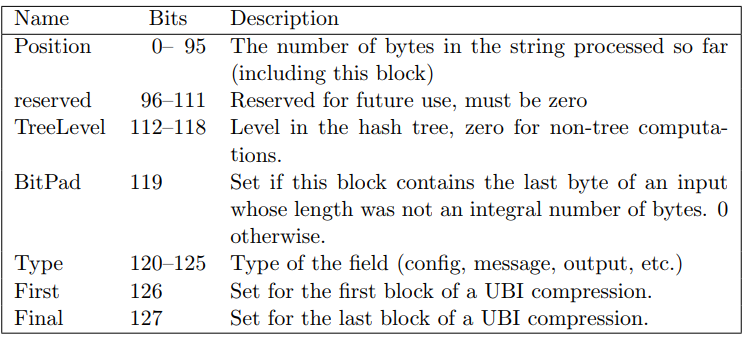
\includegraphics[width=14cm]{images/tweak.png}
\end{center}

در این جدول \lr{TreeLevel} همان \lr{bcount} است که در تابع\hyperref[subsec:skein-big-core]{\lr{skein-big-core}} در هربار صدا کردن \lr{UBI-BIG} مقدار آن یک واحد افزوده می‌شود. \lr{etype} برای رد کردن بخش \lr{position} و هم‌چنین مشخص کردن بیت \lr{first} هستند و \lr{extra} برای تعیین بیت \lr{final} و \lr{bitpad} استفاده شده‌است. پنج بیت خالی هم برای \lr{Type}قرار داده شده و هم‌چنین بخش \lr{reserved} هم صفر هست. 
\\
سپس تابع\hyperref[subsec:TFBIG-KINIT]{\lr{TFBIG-KINIT}}
صدا شده تا مقدار $ t_2 $ و $ h_8 $ برمبنای بقیه ورودی های تابع یعنی $ t_1 , t_0 $ و $ h_0 $ تا $ h_7 $ تعیین شوند. سپس برای اعداد زوج بین ۰ تا ۱۷\hyperref[subsec:TFBIG-4e]{\lr{TFBIG-4e}} و برای فردها \hyperref[subsec:TFBIG-4o]{\lr{TFBIG-4o}} صدا شده‌اند. به این ترتیب میکس در ۱۸ سری چهار تایی اجرا شده که هر کدام ۴ \lr{round} دارند و هر ۸ سری صدا شدن یکی‌است و در هر یک از این ۱۸ سری دانستن زوج و فرد بودن سری کافیست. هم‌چنین هر چهار بار یعنی در ابتدای هر ۱۷\lr{TFBIG-4e}یا\lr{TFBIG-4o} یک بار\hyperref[subsec:TFBIG-ADDKEY]{\lr{TFBIG-ADDKEY}}صدا شده تا بر مبنای شماره‌ی سری که در این‌جا با $ s$ نمایش داده شده و همین‌طور $ i $در $ pi $ و باقی مانده گرفتن از جمعشان کلید جدید مشخص شده و با \lr{pi} جمع شود. این‌جا از$ h_0 $تا$ h_7 $که حاصل سری قبلی اجرای\lr{UBI-BIG} است و همین‌طور \lr{tweak} ها استفاده شده تا مقدار جدید $ pi $ تعیین و در سری بعد استفاده شود. سپس برای بار هجدهم \lr{TFBIG-ADDKEY} صدا شده‌است. در نهایت $ hi $ از $ xor $ گرفتن $pi $ و $ mi $ به دست ‌آمده‌است. پس ‌‌‌$ hi $ نشان‌دهنده‌ی بیت‌های تغییر یافته‌ی ‌$ pi $ در طول تابع است.


\subsection{\lr{TFBIG-4e}و \lr{TFBIG-4o}}
\label{subsec:TFBIG-4e}
\label{subsec:TFBIG-4o}

این تابع برای کدگذاری $ P_0 $ تا $ P_7 $ طراحی شده‌است. همان‌طور که پیش‌تر توضیح داده شده است، ۷۲ بار تابع درهم‌سازی صدا می‌شود،‌ و هر ۸ سلسله از این ۷۲ مرحله یکسان است، هم‌چنین در هر ۸ سری ۴ بار با یک کلید و ۴ بار دیگر با یک کلید دیگر اجرا می‌شود،‌ که به همین دلیل این توابع  هر کدام برای آن ۴ باری استفاده می‌شود که در مرحله‌ای زوج یا فرد قرار داریم.
\\
این تابع یک ورودی  \lr{s} دارد. تابع  \hyperref[subsec:TFBIG-ADDKEY]{\lr{TFBIG-ADDKEY }} با ‌$ p_0 $ تا  $ p_7 $ و $ h $ و $ t $و ‌$ s $ به ترتیب به عنوان  $ w_0 $ تا $ w_7 $و $ k $و ‌$ t $ و ‌$ s $ صدا شده‌است. ‌$ h $ و $ t $ برای \lr{concat} و ساختن کلید در تابع \lr{TFBIG-ADDKEY} استفاده شده‌اند.
سپس   \hyperref[subsec:TFBIG-MIX8]{\lr{TFBIG-MIX8 }}چهار بار برای ترتیب‌های متفاوتی از ‌$ p_0 $ تا $ p_7 $ اعداد متفاوت به عنوان $ rc $ صدا شده‌است. ترتیب صدا شدن $ p_0 $ تا $ p_7 $ برای تعداد بلاک ۸ به صورت جدول‌های زیر است،‌ که برای هر ‌‌راند از ۰ تا ۳، بر حسب راند قبل ترتیب‌ها چهار عدد جابه‌جا شده‌اند. و تفاوت حالت‌های زوج و فرد در اعداد استفاده شده است.
\begin{center}
	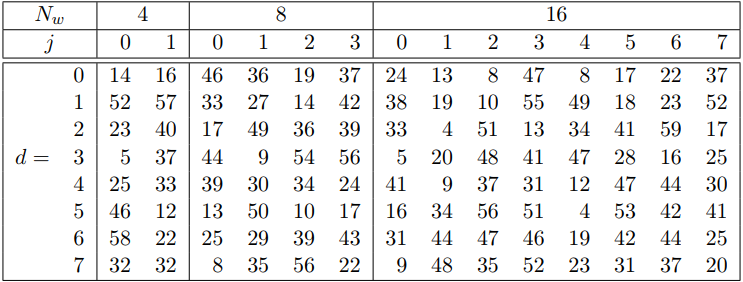
\includegraphics[width=10cm]{images/table_mix.png}
	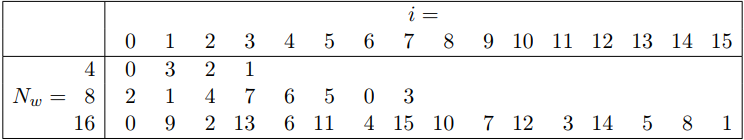
\includegraphics[width= 10cm]{images/Mix2.png}
\end{center}


\subsection{\lr{TFBIG-ADDKEY}}
\label{subsec:TFBIG-ADDKEY}

این تابع طبق فرمول‌های زیر مقادیر ورودی را تغییر می‌دهد و برای اینکار از تابع‌های \hyperref[subsec:SKBI]{\lr{SKBI}} و \hyperref[subsec:SKBT]{\lr{SKBT}} استفاده می‌کند که به ترتیب جمع مقادیر ورودی‌شان را به پیمانه ۳ و ۹ محاسبه می‌کنند.
\\متغیرهای $ h_0 $ تا $ h_8 $ در تولید کلید استفاده می‌شوند، برای محاسبه‌ی اندیس آن‌ها ( از ۰ تا ۸ ) از \lr{SKBI} استفاده شده است.
\\
متغیر‌های دیگری که در تولید کلید استفاده شده‌اند $ t_0 $ تا $ t_2 $ هستند که برای تولید اندیس آن‌ها از تابع \lr{SKBT} استفاده شده است.\\
\begin{latin}
	\begin{center}
		\begin{tabular}{c c}
			$k_{s, i} = k_{(s+i) \mod 9} $ \hspace{15mm} & $  i = 0, 1, 2, ... , 4 $ \\
			
			
		\end{tabular}
	\\
	$k_{s, 5} = k_{(s+5) \mod 9} + t_{s \mod 3}$ \\
	$k_{s, 6} = k_{(s+6) \mod 9} + t_{(s+1) \mod 3}$ \\
	$k_{s, 7} = k_{(s+7) \mod 9} + s $\\	
	\end{center}
\end{latin}

دقت شود که تمامی این محاسبات برای نوع ۵۱۲ بیتی الگوریتم است.




\subsection{\lr{SKBI}}
\label{subsec:SKBI}

تابع \lr{SKBI} برای محاسبه‌ی اندیس کلید استفاده‌ شده‌است. \\ 
در الگوریتم برای تولید $k_0 $ تا $ k_8 $ از این ماکرو استفاده شده ‌است.  ,این ماکرو $ k $ و $ s $ و $ i $ را گرفته و سپس $ k $ را به \lr{ M9-s-i }متصل می‌شود که باقی‌مانده‌ی ‌$s + i $بر ۹ تعریف شده‌است.


\subsection{\lr{SKBT}}
\label{subsec:SKBT}
برای تولید $ t_0 $ تا $ t_2 $ از این ماکرو استفاده شده است، $ t $ و $ s $ و ‌$ i $ به این تابع داده شده و سپس $ t $ به \lr{M3-s-i} متصل شده است که باقی‌مانده‌ی $ s + i $ بر ۳ تعریف شده است.

\subsection{\lr{TFBIG-MIX8}}
\label{subsec:TFBIG-MIX8}


همان‌طور که در مقدمه گفته‌ شده‌است،‌ هر سری از هشت سری، چهار \lr{round} دارد، پس طراحی این تابع برای ساده‌سازی استفاده‌ی متداول از \hyperref[subsec:TFBIG-MIX]{\lr{TFBIG-MIX}} بوده‌است. به صورت متداول در کد به چهار سری استفاده از  \lr{TFBIG-MIX}پشت سر هم نیاز است. 


\subsection{\lr{TFBIG-MIX}}
\label{subsec:TFBIG-MIX}

وظیفه‌ی این تابع درهم سازی بلاک‌های ورودی طبق فرمول‌های زیر است.
\begin{center}
	$y_0 = (x_0 + x_1) \mod 2^{64}$ \\
	$ y_1 = (x_1 <<< R_{(d \mod 8), j}) \oplus y_0$
\end{center}
که مقادیر $ R $ در جدول زیر آمده است :

\begin{center}
	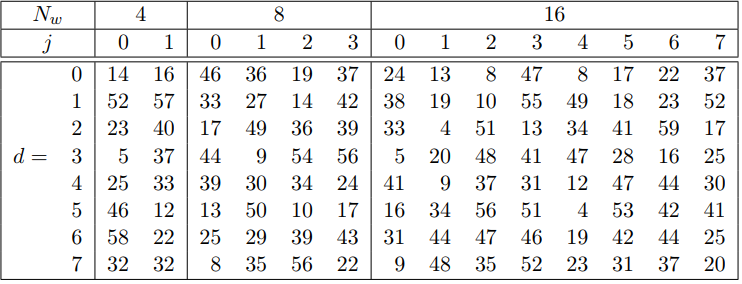
\includegraphics[width=10cm]{images/MIX1.png}
\end{center}




\subsection{\lr{TFBIG-KINIT}}
\label{subsec:TFBIG-KINIT}
این تابع با ورودی‌های $ t_0 $ تا $ t_2 $ و $h_0 $ تا $ h_8 $ مقادیر زیر را محاسبه می‌کند :
$$
k_8 = C \oplus k_0 \oplus k_1 \oplus ... \oplus k_7
$$

$$
	t_2 = t_1 \oplus t_0
$$
 که مقدار ثابت $ C $ به آن جهت در فرمول وجود دارد که از ۰ نبودن تمامی بیت‌ها اطمینان حاصل شود.
 
\subsection{\lr{DECL-STATE-BIG}} 
\label{subsec:DECL-STATE-BIG}


در این ماکرو متغیرهای ‌$ h_0 $ تا $ h_7 $ و \lr{bcount} هر دو از جنس\lr{sph-u64} (متغیر ۶۴بیتی بدون علامت) تعریف شده‌اند. 


\subsection{\lr{READ-STATE-BIG}} 
\label{subsec:READ-STATE-BIG}


این تابع برای خواندن اطلاعات از ورودی و ذخیره‌ی ‌‌آن‌ها بر روی متغیرهاست به طور دقیق‌تر  به این تابع ‌بلاک \lr{sc} به عنوان ورودی داده شده‌است. در آن متغیرهای $ h_0 $ تا $ h_7 $ و \lr{bcount} استراکت به ترتیب به متغیرهای ‌$ h_0 $ تا $ h_7 $ و \lr{bcount} ورودی مقداردهی شده‌اند.

\subsection{\lr{WRITE-STATE-BIG}} 
\label{subsec:WRITE-STATE-BIG}


این تابع برای ذخیره‌ی اطلاعات بر روی \lr{struct} است.\\
به این تابع ورودی \lr{struct}  با نام \lr{sc} داده شده‌است. متغیرهای $ h_0 $ تا $ h_7 $ و همین‌طور \lr{bcount} کد در $ h_0 $  تا  $ h_ 7 $ و \lr{bcount}  
\lr{struct}
 ذخیره شده‌اند.

\section{ توابع}

\subsection{\lr{sph-skein512-init}}
\label{subsec:sph-skein512-init}
این تابع مسئولیت مقداردهی اولیه‌ی ساختار هش را بر عهده دارد، که برای آن تابع \hyperref[subsec:skein-big-init]{\lr{skein-big-init}} را با ورودی‌ اولیه‌ی \lr{IV512} اجرا می‌کند.
\subsection{\lr{skein-big-init}}
\label{subsec:skein-big-init}

این تابع دو ورودی می‌پذیرد که یکی از آن‌ها آدرس یک ساختار هش است و دیگری مقدار اولیه، که مقادیر متناظر ساختار داده شده را برابر مقادیر اولیه قرار می‌دهد.
که مقدار اولیه در حالت ۵۱۲ بیتی در ساختار \lr{IV512} ذخیره شده ‌است.

\subsection{\lr{sph-skein512}}
\label{subsec:sph-skein512}

در این تابع ماکروی\hyperref[subsec:skein-big-core]{\lr{skein-big-core}} صدا شده‌است. ورودی‌های این تابع که بدون انجام هیچ پردازشی به \hyperref[subsec:skein-big-core]{\lr{skein-big-core}} پاس داده‌ شده‌اند،‌ ‌\lr{cc} که همان \lr{struct} شامل $h$ ها و \lr{bcount} است، \lr{data} که داده‌ی ورودی است و ‌\lr{len} که طول  \lr{data} است.


\subsection{\lr{skein-big-core}}
\label{subsec:skein-big-core}

در این تابع  همه‌ی بلاک‌های دیتا به‌جز بلاک اخر در دسته‌های ۵۱۲ تایی هش شده‌اند. مقدار ‌\lr{bcount} هم برای استفاده‌ی ثانویه تعیین شده و هم‌چنین آخرین بلاک دیتا در بافر ریخته‌ شده‌است. \\


به این تابع ورودی‌های ‌\lr{sc} که \lr{struct} شامل $ h_0 $ تا $ h_7 $ و  \lr{bcount} است، \lr{data} که داده‌ی ورودی برای هش است و \lr{len} که طول \lr{data} است پاس داده شده‌اند. در ابتدای تابع با صدا شدن \hyperref[subsec:DECL-STATE-BIG]{\lr{DECL-STATE-BIG}} متغیرهای لازم تعریف شده‌اند. سپس در یک $ if $ بررسی شده‌است که برای دیتا در بافر فضای کافی هست یا نیست: \\
- در صورتی که فضا باشد،‌ کل دیتا از جایی که پوینتر به آن اشاره کرده‌است دخیره شده‌ و سپس پوینتر که به پایان دیتای ذخیره شده اشاره دارد به اندازه‌ی طول دیتا به جلو جابه‌جا شده‌است و در خود ‌\lr{struct} هم مقدار ‌آن \lr{update} شده‌است. سپس از تابع خارج شده‌است.
\\
- در غیر این صورت، ابتدا  \hyperref[subsec:READ-STATE-BIG]{\lr{READ-STATE-BIG}} صدا شده‌است. سپس متغیر \lr{first} را به صورت یک متغیر هشت بیتی با هشت بیت ۰ یا یک بیت پرارزش یک و بقیه ۰ اند. اگر این تابع به طور متدوال از\hyperref[subsec:skein-hash]{\lr{skein-hash}}صدا شود \lr{first} برابر با ۱۲۸ می‌شود. سپس در یک لوپ ابتدا در صورت پر بودن بافر از دیتا (به این معنی که پوینتر برابر با سایز بافر شده‌باشد)،‌ اول  \lr{bcount} یکی زیاد شده‌است. سپس\hyperref[subsec:UBI-BIG]{\lr{UBI-BIG}} برای $ first + 96 $ به عنوان \lr{etype} و ۰ به عنوان \lr{extra} صدا شده‌است. پس از آن \lr{first} و \lr{ptr} هر دو صفر گذاشته شده‌اند تا برای سری بعد پر شدن دیتا بافر از ابتدا \lr{overwrite} شود. سپس شرط پر بودن بافر تمام شده و به اندازه‌ی مینیموم مقداری که در بافر جا هست با طول دیتای باقی‌مانده در بافر دیتا ذخیره شده‌است. پوینتر و دیتا با مقدار این مینیموم جمع و \lr{len} منهای آن شده‌ تا مقدار دیتای باقی‌مانده را نشان دهد. و سپس حلقه تکرار تا زمانی که هنوز دیتایی باقی مانده‌باشد تکرار می‌شود. درواقع در این حلقه هر سری به تعداد بزرگترین مضرب سایز بافر که کوچک‌تر از \lr{len} دیتا است روی همان طول از دیتا \hyperref[subsec:UBI-BIG]{\lr{UBI-BIG}} صدا شده‌است. \lr{bcount} همین تعداد بار را نشان می‌دهد. برای آخرین سری که مضرب کاملی از بافر نیست تنها دیتای باقی‌مانده در بافر ذخیره شده و \lr{ptr} به آخر آن اشاره کرده‌است. 
در آخر \hyperref[subsec:WRITE-STATE-BIG]{\lr{WRITE-STATE-BIG}}
صدا و بعد مقدار فعلی پوینتر هم در \lr{struct} ذخیره شده‌است. 
نحوه ذخیره‌سازی \lr{tweak} به شکل زیر است. 
\begin{center}
	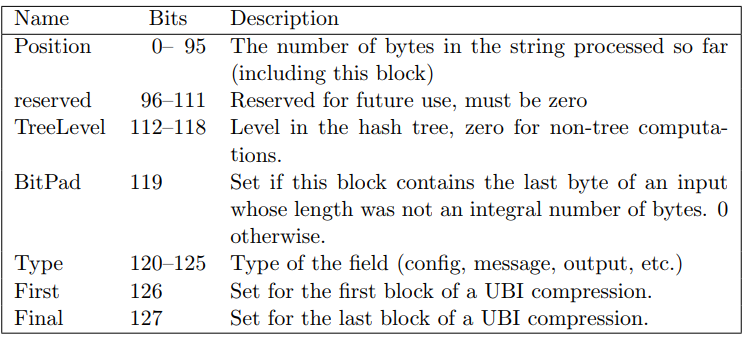
\includegraphics[width=14cm]{images/tweak.png}
\end{center}

دلیل جمع کردن \lr{first} با ۹۶،‌ رد کردن بخش \lr{position} است. حالت اولیه \lr{first} هم به این علت با چک کردن \lr{bcount} مقداردهی شده که مقدار بخش \lr{first} باید برای سری اول گرفتن بلوک دیتا برابر با ۱ باشد. 

در این تابع ممکن است سایز دیتا دقیقا مضربی از سایز بلاک (۵۱۲) باشد،‌ برای این حالت باید مقدار بیت فیلد \lr{final} یک شود. اما این تابع از این که در حال پردازش اخرین بخش دیتا هست یا نه باخبر نیست و درنتیجه در‌ آخر ممکن است بافر شامل یک بلاک کامل از دیتا باشد. 



\subsection{\lr{skein-hash}}
\label{subsec:skein-hash}

در این تابع ابتدا هش از جنس آرایه‌ای ۶۴ تایی از کاراکتر‌های بدون علامت (\lr{uint8-t}) و سپس \lr{struct} \lr{ctx} از جنس \hyperref[subsec:sph-skein-big-context]{\lr{sph-skein-big-context}} تعریف شده‌است. این هش ۵۱۲ در ۵۱۲ است و به همین دلیل حاصل نهایی هم ۶۴ بایت درنظر گرفته شده. سپس آدرس \lr{ctx} به تابع\hyperref[subsec:sph-skein512-init]{\lr{sph-skein512-init}} پاس داده شده‌است. در این تابع مقدارهای اولیه در ‌\lr{struct} ذخیره شده‌است. سپس تایع \hyperref[subsec:sph-skein512]{\lr{sph-skein512}} صدا شده که در آن تمام بلاک‌های دیتا به جز بلاک آخر صدا و بلاک ‌اخر هم در بافر ذخیره شده‌است. سپس تابع  \hyperref[subsec:sph-skein512-close]{\lr{sph-skein512-close}} صدا شده و به آن ‌\lr{struct} و ادرس شروع \lr{hash} داده شده‌است. در این مرحله بیت‌های اضافی اضافه، بلاک ‌آخر هش و در ‌\lr{dst} ذخیره شده‌اند. 
در نهایت ۳۲ بایت از \lr{hash} در \lr{output} ریخته شده‌اند.

\subsection{\lr{sph-skein512-close}}
\label{subsec:sph-skein512-close}

